\documentclass{article}
\usepackage[utf8]{inputenc}
\usepackage[margin=1in]{geometry}
\usepackage{fancyhdr}
\usepackage{graphicx}
\usepackage{listings}
\usepackage{parskip}

\makeatletter
  \def\@seccntformat#1{\@ifundefined{#1@cntformat}
    {\csname the#1\endcsname\space}
    {\csname #1@cntformat\endcsname}}
  \newcommand\section@cntformat{\thesection.\space}       
  \newcommand\subsection@cntformat{\thesubsection.\space}
\makeatother

\newcommand{\code}[1]{\texttt{#1}}

\renewcommand\thesubsection{\alph{subsection}}

\title{EECS 219C: Formal Methods — Assignment 2}
\author{Parker Ziegler}
\pagestyle{fancy}
\lhead{EECS 219C: Formal Methods — Assignment 2}
\rhead{Parker Ziegler}

\begin{document}

\maketitle

\section{Bit Twiddling Hacks}

\subsection{Equivalence of \code{f1} and \code{f2}}

My SMT-LIB encoding to check equivalence of \code{f1} and \code{f2} is located in \code{1a.smt2}. Based on my encoding, \code{f1} and \code{f2} \textbf{are not equivalent}. Z3 provides the counterexample $x = 1$, in which \code{f1(x)} evlauates to -1 while \code{f2(x)} evaluates to 1. The full output returned by Z3 is:

\begin{lstlisting}
(
  (define-fun v_1 () (_ BitVec 32)
    #x00000000)
  (define-fun x () (_ BitVec 32)
    #x00000001)
  (define-fun v_0 () (_ BitVec 32)
    #xffffffff)
  (define-fun ret_2 () (_ BitVec 32)
    #x00000001)
  (define-fun v_2 () (_ BitVec 32)
    #x00000001)
  (define-fun ret_1 () (_ BitVec 32)
    #xffffffff)
)
\end{lstlisting}

A more readable output provided by Z3 using its Python API yields the following \code{list} showing assignments in the counterexample:

\begin{lstlisting}[language=Python]
[x = 1, v_0 = -1, ret_1 = -1, v_1 = 0, v_2 = 1, ret_2 = 1]
\end{lstlisting}

\subsection{Equivalence of \code{f3} and \code{f4}}

My SMT-LIB encoding to check equivalence of \code{f3} and \code{f4} is located in \code{1b.smt2}. Based on my encoding, \code{f3} and \code{f4} \textbf{are equivalent}.

\subsection{Synthesizing an equivalent function for \code{f2} without bit-wise operators}

To synthesize an equivalent function for \code{f2}, we use syntax-guided synthesis (SyGuS) with Linear Integer Arithmetic (LIA) as the underlying theory. My encoding of the synthesis problem in SyGuS-IF format is located in \code{1c.sy}. I used the CVC4 solver to synthesize the following solution.

\begin{lstlisting}
(define-fun f2Equiv ((x Int)) Int (ite (<= 0 x) x (- 0 x)))
\end{lstlisting}

I restricted the grammar to basic arithmetic operators, conditionals, and arithmetic comparators. Reading through the implementation of \code{f2}, I inferred that it returns as output the absolute value of its input \code{x}. Therefore, I used the constraint \code{(= (f2Equiv x) (abs x))} to describe the semantics of the function we aim to synthesize.

\section{Sum-Sudoku}

\subsection{Formulate an SMT instance that finds a solution to Sum-Sudoku puzzles}

My encoding of the Sum-Sudoku problem is located in \code{sumsudoku.py}. My encoding applies the following constraints:

\begin{enumerate}
  \item Ensure that every integer in a row is distinct; that is, the same integer cannot appear twice in a given row. We encode this using \code{z3.Distinct}.
  \item Ensure that every integer in a column is distinct; as above, we encode this with \code{z3.Distinct}.
  \item Ensure that all values in a row sum up to their required row sum. We encode this using \code{z3.Sum} to sum variables and compare the resulting value using numerical equality to its row sum (which is given).
  \item Ensure that all values in a column sum up to their required column sum. As above, we use \code{z3.Sum}.
\end{enumerate}

We apply the theories of equality and uninterpreted functions (EUF) and linear integer arithmetic (LIA) to specify these constraints. EUF can be used to represent the \code{z3.Distinct} API; for example, we can think of \code{z3.Distinct(x, y, z)} as a conjunction of pairwise disequalities $x \neq y \land y \neq z \land x \neq z$. We use LIA as the underlying theory for \code{z3.Sum}.

\subsection{Assigning row and column sum values for a unique Sum-Sudoku problem}

In order to find an assignment to row and column sums such that the resulting Sum-Sudoku problem has a unique solution, we need to articulate what ``uniqueness" means in this context.


In first-order logic, the symbol $\exists!$ articulates the idea that a \emph{unique} value exists that makes a given proposition true. We can model $\exists!$ using the following logical equivalence:

$$
\exists!~x.P(x) \iff \exists x.(P(x) \land \forall y.(P(y) \Longrightarrow y = x))
$$

My encoding applies this process of uniqueness quantification in the following ways:

\begin{enumerate}
  \item Declares a new set of Z3 variables (\code{rs\_y}, \code{cs\_y}, \code{grid\_y}, \code{vs\_y}) to represent $y$ in the above first-order logic statement.
  \item Uses the \code{z3.ForAll} universal quantifier to search for row sums \code{rs\_y} and column sums \code{cs\_y} that satisfy the following implication:
  \begin{enumerate}
    \item \textbf{If} \code{valid((rs\_y, cs\_y, grid\_y, vs\_y))} — the puzzle is valid when applied to the new variables representing $y$.
    \item \textbf{Then} \code{pairwise\_equal(rs + cs, rs\_y + cs\_y)} — the row sums and column sums found for puzzle $y$ are identical to those for puzzle $x$ and, thus, correspond to assignments for a unique puzzle.
  \end{enumerate}
\end{enumerate}

\textbf{Examining solver runtimes for varying values of $m$ and $n$}

If we increase $m$ and $n$ linearly with one another, we find that solver time appears to follow a pattern of exponential growth. Figure \ref{fig:sumsudoku} plots the running times for our puzzle creation algorithm on inputs $(m, n)$ from $(5, 3)$ to $(15, 13)$; $m$ and $n$ are both increased linearly in each run. Figure \ref{fig:sumsudoku-log} plots $log(runtime)$ for the same inputs. The trend for $log(runtime)$ appears to be somewhere between logarithmic and linear, suggesting that the algorithm in the best case runs in polynomial time and, in the worst case, exponential time.

\begin{figure}
  \centering
  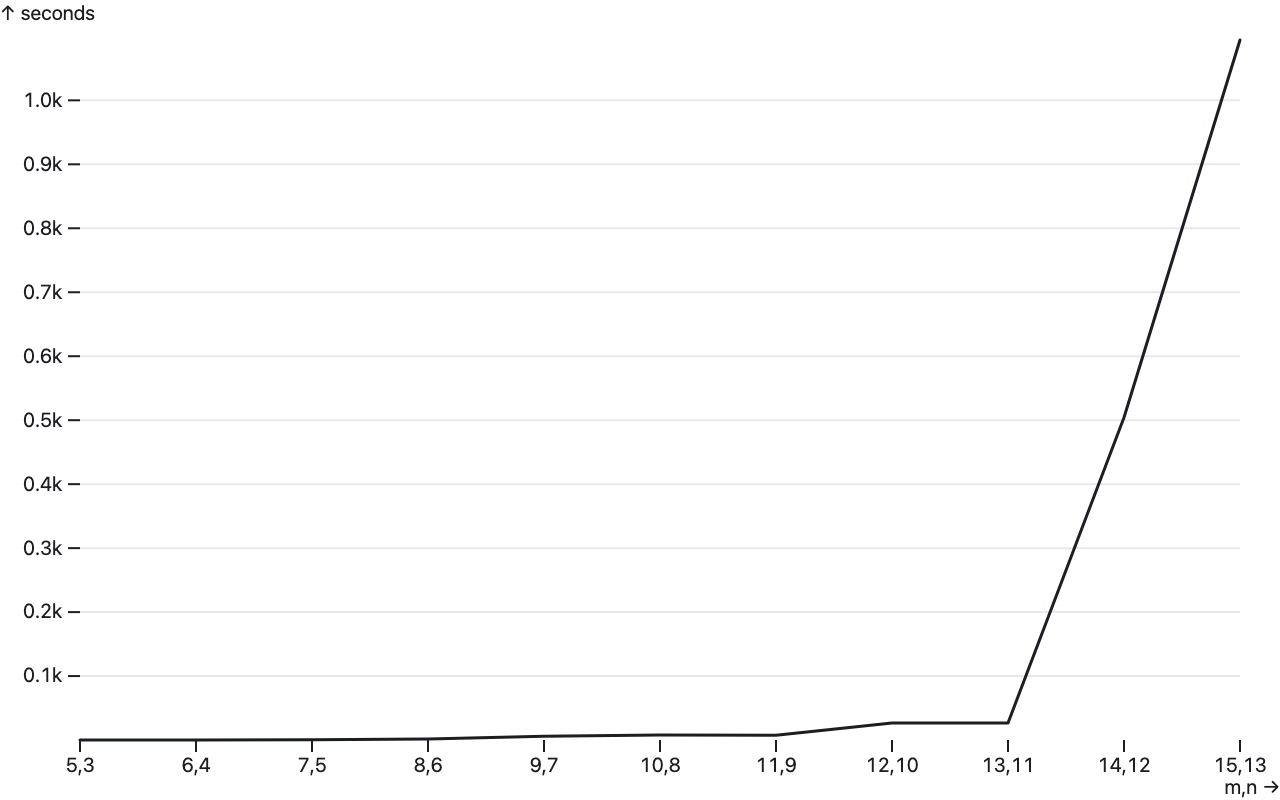
\includegraphics[width=0.9\textwidth]{sumsudoku}
  \caption{The relationship between the max allowed cell value $m$, the size of the grid $n$, and the running time of Z3 to find a unique puzzle.}
  \label{fig:sumsudoku}
\end{figure}

\begin{figure}
  \centering
  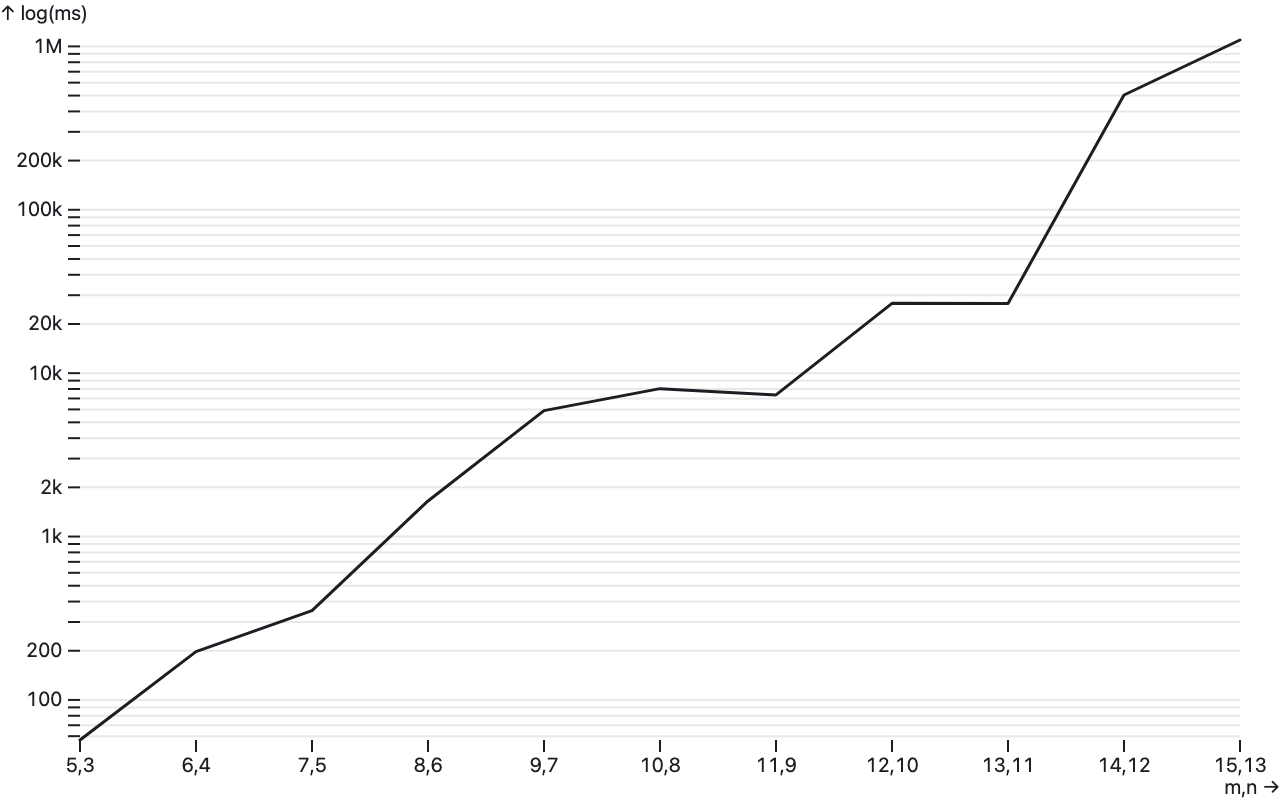
\includegraphics[width=0.9\textwidth]{sumsudoku-log}
  \caption{The relationship between the max allowed cell value $m$, the size of the grid $n$, and $log$ of the running time of Z3 to find a unique puzzle.}
  \label{fig:sumsudoku-log}
\end{figure}

\subsection{Making unique Sum-Sudoku puzzles by emptying cells}

My encoding of the algorithm to make a unique Sum-Sudoku puzzle by gradually emptying cells and checking that the resulting puzzle is unique is encoded in \code{makepuzzleunique.py}. My algorithm works using the following strategy.

\begin{enumerate}
  \item Start with a fully filled out Sum-Sudoku grid, which by definition is a unique solution.
  \item Enter into a \code{while} loop guarded by a flag \code{solution\_unique}, which is initially set to \code{True}.
  \item Create a set of constraints that ensure the following properties:
  \begin{enumerate}
    \item All row sum and column sum variables must be equal to their values in the initial unique solution.
    \item All cell variables must be equal to their values in the initial unique solution \textbf{if they have not been emptied}.
    \item The puzzle must be valid according to the implementation of \code{valid} from Part A.
  \end{enumerate}
  \item We then check if our set of constraints has \emph{exactly one solution}. This is accomplished by:
  \begin{enumerate}
    \item Finding the first model that satisfies the constraints.
    \item For each assignment in the model, negating its assignment and adding it as an additional constraint. This ensures that the current model will no longer be valid on subsequent iterations.
    \item Iterating until we either no longer find a satisfying assignment or we've exceeded our \code{max\_models}, which in this case is 1.
  \end{enumerate}
  \item If our model has exactly one solution, we pick a cell at random to ``empty" and track it in the list \code{cells\_emptied}. We also store the unique model and compute the new value of the \code{flags} list.
  \item We repeat steps 3 and 4 until we hit a case where our model has more than one solution, at which point we set \code{solution\_unique} to \code{False} and exit the \code{while} loop.
  \item The variable \code{last\_unique\_model} stores the last model that had a unique solution. The variable \code{flags} is computed by creating a list of length \code{n * n - 1} and filling it with \code{True} if the cell at index \code{i} is not empty in the model and \code{False} if it is.
\end{enumerate}

In general, the algorithm works off of the idea that, if we find a solution after emptying a cell, we can negate the assignment to grid cells in that model to ``block'' Z3 from exploring that model again. This is what allows us to determine if a given state of the partially filled-out grid can be completed in more than one way, at which point the puzzle would cease to have a unique solution.

\section{Bag of Chips}

\subsection{Prove that the choose-and-replace process on the bag of chips always halts}

Our goal is to show that you can only execute the described choose-and-replace process on our bag of chips a finite number of times. To do this, we define a relation $<_{ybr}$ over our state tuples $(\#red_i, \#blue_i, \#yellow_i)$. Our relation has the following semantics:


$(\#red_{i + 1}, \#blue_{i + 1}, \#yellow_{i + 1}) <_{ybr} (\#red_i, \#blue_i, \#yellow_i)$ iff

\begin{enumerate}
  \item $\#yellow_{i + 1} < \#yellow_i$, OR
  \item $\#yellow_{i + 1} = \#yellow_i \land \#blue_{i + 1} < \#blue_i$, OR
  \item $\#yellow_{i + 1} = \#yellow_i \land \#blue_{i + 1} = \#blue_i \land \#red_{i + 1} < \#red_i$
\end{enumerate}

To prove termination, we need to show that for an arbitrary state $(\#red_i, \#blue_i, \#yellow_i)$, a finite number of choose-and-replace operations remain; that is, that $<_{ybr}$ is a well-founded relation with no infinite descending chains. The proof is by induction on the triple $(\#red_i, \#blue_i, \#yellow_i)$.

\textbf{Base Case}

There are four base cases to consider. If $(\#red_i, \#blue_i, \#yellow_i)$ is equal to $(0, 0, 0)$, the process has terminated. If $(\#red_i, \#blue_i, \#yellow_i)$ is in the set $\{(0, 0, 1), (0, 1, 0), (1, 0, 0)\}$, then only one step remains — removing the last chip from the bag. This proves termination of the base case.

\textbf{Inductive Step}

We take as the inductive hypothesis that for any state $(\#red_i, \#blue_i, \#yellow_i)$, the $i + 1$ state:

$$(\#red_{i + 1}, \#blue_{i + 1}, \#yellow_{i + 1})$$

only has a finite number of choose-and-replace operations that remain. We now apply case analysis based on the semantics of the choose-and-replace operation.

\emph{Case 1: One of the removed chips is red}

Starting from an arbitrary state $(\#red, \#blue, \#yellow)$ and removing at least one red chip from the bag yields one of three possible states:

\begin{enumerate}
  \item $(\#red - 1, \#blue - 1, \#yellow)$
  \item $(\#red - 1, \#blue, \#yellow - 1)$
  \item $(\#red - 2, \#blue, \#yellow)$
\end{enumerate}

The second restriction of the semantics of the $<_{ybr}$ relation shows that:

$$
(\#red - 1, \#blue - 1, \#yellow) <_{ybr} (\#red, \#blue, \#yellow)
$$

The first restriction shows that:

$$
(\#red - 1, \#blue, \#yellow - 1) <_{ybr} (\#red, \#blue, \#yellow)
$$

Finally, the third restriction shows that:

$$
(\#red - 2, \#blue, \#yellow) <_{ybr} (\#red, \#blue, \#yellow)
$$

Therefore, all new states abide by our well-founded relation for the first case.

\emph{Case 2: Both of the removed chips are yellow}

Starting from an arbitrary state $(\#red, \#blue, \#yellow)$ and removing two yellow chips from the bag yields a new state $(\#red, \#blue + 5, \#yellow - 1)$. By the first resitrction of the semantics of the $<_{ybr}$ relation, we can indeed see that:

$$
(\#red, \#blue + 5, \#yellow - 1) <_{ybr} (\#red, \#blue, \#yellow)
$$

\emph{Case 3: One of the removed chips is blue}

Starting from an arbitrary state $(\#red, \#blue, \#yellow)$ and removing one blue chip from the bag yields one of two potential states:

\begin{enumerate}
  \item $(\#red + 10, \#blue - 2, \#yellow)$
  \item $(\#red + 10, \#blue - 1, \#yellow - 1)$
\end{enumerate}


For the first case, the second restriction of the semantics of the $<_{ybr}$ relation allow us to conclude that:

$$
(\#red + 10, \#blue - 2, \#yellow) <_{ybr} (\#red, \#blue, \#yellow)
$$

For the second case, the firt restriction of the semantics of the $<_{ybr}$ relation allow us to conclude that:

$$
(\#red + 10, \#blue - 1, \#yellow - 1) <_{ybr} (\#red, \#blue, \#yellow)
$$

In all cases, we've shown that:

$$
(\#red_{i + 1}, \#blue_{i + 1}, \#yellow_{i + 1}) <_{ybr}(\#red_i, \#blue_i, \#yellow_i)
$$

This completes the inductive argument and, with it, the proof of termination.

\subsection{Prove that the variant of the bag of chips problem always halts}

Our goal is the same as in part (a), but we need to modify our relation slightly to prove termination in this variant of the bag of chips problem. We define this new relation, $<_{ryb}$, to have the following semantics:

$(\#red_{i + 1}, \#blue_{i + 1}, \#yellow_{i + 1}) <_{ryb} (\#red_i, \#blue_i, \#yellow_i)$ iff

\begin{enumerate}
  \item $\#red_{i + 1} < \#red_i$, OR
  \item $\#red_{i + 1} = \#red_i \land \#yellow_{i + 1} < \#yellow_i$, OR
  \item $\#red_{i + 1} = \#red_i \land \#yellow_{i + 1} = \#yellow_i \land \#blue_{i + 1} < \#blue_i$
\end{enumerate}

This relation is similar to $<_{ybr}$ with the exception of comparison order. While $<_{ybr}$ compares values of two state triples in the order yellow $\rightarrow$ blue $\rightarrow$ red, our new relation $<_{ryb}$ compares these values in the order red $\rightarrow$ yellow $\rightarrow$ blue. As above, our proof is by induction on the triple $(\#red_i, \#blue_i, \#yellow_i)$.

\textbf{Base Case}

The base case is identical to the proof in (a); therefore, we elide it here.

\textbf{Inductive Step}

Again we take as the inductive hypothesis that for any state $(\#red_i, \#blue_i, \#yellow_i)$, the $i + 1$ state:

$$(\#red_{i + 1}, \#blue_{i + 1}, \#yellow_{i + 1})$$

only has a finite number of choose-and-replace operations that remain. We now apply case analysis based on the semantics of the choose-and-replace operation.

\emph{Case 1: One of the removed chips is red and the other is yellow}

Starting from an arbitrary state $(\#red, \#blue, \#yellow)$ and removing one yellow chip and one red chip yields a new state $(\#red, \#blue, \#yellow - 1)$. By the second restriction of the semantics of the $<_{ryb}$ relation, we can see that:

$$
(\#red, \#blue, \#yellow - 1) <_{ryb} (\#red, \#blue, \#yellow)
$$

\emph{Case 2: Both removed chips are yellow}

Starting from an arbitrary state $(\#red, \#blue, \#yellow)$ and removing two yellow chips yields a new state $(\#red , \#blue + 5, \#yellow - 2)$. By the second restriction of the semantics of the $<_{ryb}$ relation, we can see that:

$$
(\#red, \#blue + 5, \#yellow - 2) <_{ryb} (\#red, \#blue, \#yellow)
$$

\emph{Case 3: One of the removed chips is blue and the other is red}

Starting from an arbitrary state $(\#red, \#blue, \#yellow)$ and removing one blue chip and one red chip yields a new state $(\#red - 1, \#blue + 9, \#yellow)$. By the first restriction of the semantics of the $<_{ryb}$ relation, we can see that:

$$
(\#red - 1, \#blue + 9, \#yellow) <_{ryb} (\#red, \#blue, \#yellow)
$$

This completes the inductive argument and, with it, the proof of termination.

\subsection{Pitfalls of using conjunctions to represent implications in SMT solvers}

Using the strategy of asserting $A_1, A_2,..., A_k, \lnot B$, checking if its conjunction is SAT, and taking UNSAT to mean that $(A_1 \land A_2 \land ... \land A_k) \Longrightarrow B$ runs into issues in cases where $A_i$ is incorrectly encoded.

Consider the case where $A_i$ is incorrectly encoded such that it evaluates to $false$. Our conjunction $A_1, A_2,..., A_k, \lnot B$ would then evaluate to $false$ (UNSAT) regardless of the value of $\lnot B$. In this case, we would erreonously consider our original proposition ($A_1 \land A_2 \land ... \land A_k) \Longrightarrow B$ to be proven; in essence, a \emph{false positive}.

Now consider the case where $A_i$ is incorrectly encoded such that it evaluates to $true$. Our conjunction $A_1, A_2,..., A_k, \lnot B$ \emph{may} evaluate to $true$ (SAT) or $false$ (UNSAT) depending on the values of all other $A_{1..k}$ and $B$. The negative impact in this case is that, if $A_i$ evaluates to $true$ when it shouldn't, our conjunction could \emph{also} evaluate to $true$ (SAT) when it shouldn't. This would lead us to believe that our original proposition ($A_1 \land A_2 \land ... \land A_k) \Longrightarrow B$ is disproven; in essence, a \emph{false negative}.

In order to mitigate the impact of an incorrect encoding $A_i$, we could consider rewriting our implication using the rule of inference. The rule of inference states that:

$$
P \Longrightarrow Q \iff \lnot P \lor Q
$$

Applying this to our implication results in $\lnot A_1 \lor \lnot A_2 \lor...\lor \lnot A_k \lor B$. Now, if $A_i$ incorrectly evaluates to $false$, it does not immediately make the entire disjunction SAT or UNSAT — we still must take all other theory literals into account, including $B$, to determine if there is a satisfying assignment. Recall that before, in the case when $A_i$ incorrectly evaluated to $false$, the unsatisfiability of our conjunction was guaranteed regardless of the value of $\lnot B$. In essence, we've limied the ability of a single incorrect encoding to influence the determination of SAT or UNSAT.

\end{document}